\documentclass[conference,onecolumn]{IEEEtran}

\usepackage{cite}
\usepackage[pdftex]{graphicx}
\graphicspath{{figures/}}
\usepackage[cmex10]{amsmath}
\usepackage{algorithmic}
\usepackage{algorithm}
\usepackage{array}
\usepackage{fixltx2e}
\usepackage{stfloats}
\usepackage{url}
\usepackage{amssymb}
\usepackage{float}
\usepackage{color}
\usepackage{balance}
\usepackage{subfig}
\usepackage{multirow}
\usepackage[margin=1in]{geometry}
\usepackage{placeins} %enables float barrier
%\usepackage{caption} %uncomment these for more space between a table and its caption
%\captionsetup[table]{skip=5pt}

\newcommand{\norm}[1]{\left\lVert #1 \right\rVert}

\begin{document}

\title{Training Stacked Denoising Autoencoders for Representation Learning}

\author{\IEEEauthorblockN{Jason Liang}
\IEEEauthorblockA{jasonzliang@utexas.edu}
\and
\IEEEauthorblockN{Keith Kelly}
\IEEEauthorblockA{keith@ices.utexas.edu}}

\maketitle

\begin{abstract}
We implement stacked denoising autoencoders, a class of neural networks that are capable of learning powerful representations of high dimensional data. We describe stochastic gradient descent for unsupervised training of autoencoders, as well as a novel genetic algorithm based approach that makes use of gradient information. We analyze the performance of both optimization algorithms and also the representation learning ability of the autoencoder when it is trained on standard image classification datasets. 
\end{abstract}

\FloatBarrier
\section{Introduction}
Autoencoders are a method for performing representation learning, an unsupervised pretraining process during which a more useful representation of the
input data is automatically determined. Representation learning is important in machine learning since ``the performance of 
machine learning methods is heavily dependent on the choice of data representation (or features) in which they are applied" 
\cite{bengio2012rep}. For many supervised classification tasks, the high dimensionality of the input data means that the classifier requires an enormous number of training examples in order to generalize well and not overfit. One solution is to use unsupervised pretraining to learn a good representation for the input data and during actual training, transform the input examples into an easier form for the classifier to learn. Autoencoders are one such representation learning tool.

An autoencoder is a neural network with a single hidden layer and where the output layer and the input layer have the same size. Suppose that the input $x\in\mathbb{R}^m$ (and the output as well) and suppose that the hidden layer has $n$ nodes. Then we have a weight matrix $W\in\mathbb{R}^{m\times n}$ and bias vectors $b$ and $b^{'}$ in $\mathbb{R}^m$ and $\mathbb{R}^n$, respectively. Let $s(x) = 1/(1+e^{-x})$ be the sigmoid (logistic) transfer function. Then we have a neural network as shown in Fig.~\ref{fig:autoencoder}. When using an autoencoder to encode data, we calculate the vector $y=s(Wx + b)$; corresponding when we use an autoencoder to decode and reconstruct back the original input, we calculate $z=s(W^{T}x+b^{'})$. The weight matrix of the decoding stage is the transpose of weight matrix of the encoding stage in order to reduce the number of parameters to learn. We want to optimize $W$, $b$, and $b^{'}$ so that the reconstruction is as similar to the original input as possible with respect to some loss function. In this report, the loss function used is the least squares loss: $E(t,z)=\frac{1}{2}\norm{t-z}_2^2$, where $t$ is the original input. After an autoencoder is trained, its decoding stage is discarded and the encoding stage is used to transform the training input examples as a preprocessing step. We will refer to the trained encoding stage of the autoencoder as an ``autoencoder layer".  

For ordinary autoencoders, we usually want that $n<m$ so that the learned representation of the input exists in a lower dimensional space than the input. This is done to ensure that the autoencoder does not learn a trivial identity transformation. However, there also exists an autoencoder variant called \textit{denoising autoencoders} that use a different reconstruction criterion to learn overcomplete representations \cite{vincent2010stacked}. In other words, even if $n>m$, a denoising autoencoder can still learn a good representation of the input. This is achieved by corrupting the input image and training the autoencoder to reconstruct the original uncorrupted image. By learning how to denoise, the autoencoder is forced to understand the true structure of input data and learn a good representation of it. 

We will consider training denoising autoencoders with stochastic gradient descent (SGD). Background literature for denoising autoencoders can be found in the related work section. The algorithm description section contains more details about how SGD is implemented for autoencoders. The experiments section describes the results of training an autoencoder on a handwritten digit image dataset. Finally in future work, we discuss our plans to improve upon existing training algorithms.


\FloatBarrier
\section{Related Work}
Dimensionality reduction of high dimensional data is a common problem in machine learning with many applications. Given input points embedded in high dimensional space, the goal of dimensionality reduction is to learn a lower dimensional manifold that fits most of the points well. Simpler methods such as principal component analysis (PCA) \cite{wold1987principal} work by finding the orthogonal directions that best explains the variance of the input data. These directions or ``principal components'' can be then used to transform the input data by mapping it to coordinates along the principal components. The main drawback of PCA is that it only learn a linear transformation, which means PCA performs poorly when the input data do not lie on a linear manifold (a hyperplane). More sophisticated variants such as kernel PCA \cite{scholkopf1997kernel} deal with nonlinear input by using a nonlinear transformation to map the input data points into a higher dimensional space where they are approximately linear. Other nonlinear manifold learning algorithms include Isomap \cite{tenenbaum2000global} and t-SNE \cite{van2008visualizing}. These algorithms use heuristics to compute a similarity metric between the input points and then perform multidimensional scaling. Unfortunately, all of these methods mentioned above only work well if the manifold is locally smooth and often degrade in performance for highly varying manifolds \cite{van2008visualizing}.

Autoencoders, also known as auto-associators, are a class of feed-forward neural networks that are designed for performing dimensionality reduction and manifold learning \cite{hinton2006reducing}. Artificial neural networks are biologically inspired computational structures that are capable of approximating functions of arbitrary shape and dimensionality \cite{haykin2004comprehensive}. Unlike normal neural networks for regression or classification, autoencoders are trained in an unsupervised manner. The weights of an autoencoder can be trained with any optimization algorithm, but the mostly commonly used one is gradient descent, also known as the backpropagation algorithm \cite{hecht1989theory,bottou-91c}. 

Most recent research on autoencoders focus on training them to perform representation learning \cite{bengio2012rep}. Representation learning is a generalization of manifold learning where the goal is not only to discover a lower dimensional substructure, but also to learn a higher dimensional but sparser and more linearly separable representation of the input data. It has been shown that training autoencoders to denoise is one way to learn good representations of the data \cite{vincent2010stacked}. Similarly, adding a regularization term that penalizes the Frobenius norm of the Jacobian matrix of the encoder activations is also effective \cite{rifai2011contractive}. Furthermore, by stacking autoencoders, it has been shown that the resulting deep neural network is able to overcome the difficulties associated with existing dimensionality reduction methods in learning highly varying manifolds \cite{van2008visualizing,vincent2010stacked}.

A related research area to representation learning is deep learning, where deep neural networks are trained such that each subsequent layer learns a higher level representation of the input of the previous data \cite{bengio2009learning}. It has been shown with each additional layer, the transformed input feature steadily becomes more global and less invariant to local distortions. Compared to shallow neural networks, deep neural networks perform and generalize better on classification tasks, especially for high dimensional inputs. In fact for many standard datasets, their performance is state of the art by a wide margin \cite{schmidhuber2014deep}. 

Besides stacked autoencoders, the other two major deep learning architectures are stacked restricted Boltzmann machines (RBMs) \cite{hinton2006fast} and convolutional neural networks (CNNs) \cite{lecun1995convolutional}. A RBM is a undirected graphical model that is trained to learn the distribution of the input data. The special bipartite structure of the RBM makes Gibbs sampling tractable and gives rise to a fast training algorithm called contrastive divergence \cite{hinton2006fast,hinton2006learning}. Like autoencoders, RBMs can also be stacked in a similar manner and converted into a deterministic deep neural network \cite{hinton2006reducing}. CNNs are a type of deep neural network that is especially designed for processing image data and are composed of two main types of layers: convolutional and max pooling. In the convolutional layer, local filters of weights are convolved with the input while in the max pooling layer, the input is down-sampled. CNNs are trained in a supervised manner with backpropagation. Due to the sparsity of the architecture, CNNs can be efficiently trained for input data with millions of dimensions and consequently, achieve state of the art performance in many large scale image classification benchmarks \cite{ciresan2011committee,krizhevsky2012imagenet,goodfellow2013multi}.

A survey of GAs and how they perform optimization can be found in \cite{srinivas1994genetic}. Much research has be done in applying GAs for optimization of weights in neural networks \cite{gomez2006efficient,floreano2008neuroevolution}. There is a small amount of recent work on applying GAs and evolutionary algorithms in general to deep learning \cite{koutnik2014evolving,david2014genetic}. Cant{\'u}-Paz discusses methods for parallelizing GAs, which will be essential to scalability when using a GA to train our autoencoder \cite{cantu1998survey}.


\FloatBarrier
\section{Algorithm Description}
\subsection{Stochastic Gradient Descent}

We start with a random weight matrix $W$ and random biases $b$ and $b^{'}$. We take a given input $x$, and feed it forward through the network and compute the error between the target output $t$ and the actual output $z$. Often we use the squared loss error $E(t,z) = \frac{1}{2}\norm{t-z}_2^2$ to determine the difference between the two. In the case of an autoencoder, the target output is the same as the input. If the error is not satisfactory, we can adjust the weight matrix and that biases in order to attempt to learn a better representation of the data. A common method of updating the weight and biases is via backpropagation \cite{hecht1989theory}; when applied to training inputs one at a time, it is also known as stochastic gradient descent (SGD). We will first consider the update for the weights and biases from the last hidden layer to the output layer with a squared loss error function and derive the updates. We use as an example a simple three layer neural network (input, one hidden and output layer). Some notation is given in Table \ref{tab:notation}.

\begin{table}[h]
	\centering
\begin{tabular}{l|l}
Symbol     & Meaning                                                          \\ \hline
$E$          & Error as computed at the output layer                            \\
$x_j$       & Node $j$ in the input layer                                      \\
$y_j$       & Node $j$ in the hidden layer                                     \\
$z_j$       & Node $j$ in the output layer                                     \\
$n_j$       & $\sum_{i=1}^n W_{ij}x_i + b_j$                                   \\
$t_j$       & Target output at node $j$                                   \\
$W_{ij}^H$ & Weight $i,j$ from input to hidden layer \\
$W_{ij}^O$ & Weight $i,j$ from hidden to output layer \\
$s(x_j)$    & $1/(1+e^{-x_j})$                                                 \\
$b_j^{\{H,O\}}$    & Biases for hidden and output layer                                                \\
\end{tabular}
\caption{Table giving notation for the derivation of updates.}
\label{tab:notation}
\end{table}

The derivative of the output error $E$ with respect to an output matrix weight $W_{ij}^O$ is as follows.

\begin{equation}
\begin{split}
\frac{\partial E}{\partial W^O_{ij}} &= \frac{\partial E}{\partial z_j}\frac{\partial z_j}{\partial W^O_{ij}} \\
																	 &=(z_j - t_j)\frac{\partial s(n_j)}{\partial x_j}\frac{\partial x_j}{\partial W^O_{ij}} \\
																	 &=(z_j-t_j)s(n_j)(1-s(n_j))x_i \\
																	 &=(z_j-t_j)z_j(1-z_j)x_i \\
\end{split}
\label{}
\end{equation}
Now that we have the gradient for the error associated to a single training example, we can compute the updates.
\begin{equation}
\begin{split}
\delta^O_j &= (z_j-t_j)z_j(1-z_j) \\
W^O_{ij} &\leftarrow W^O_{ij} - \eta \delta^O_j x_i \\
b^O_j &\leftarrow b^O_j - \eta\delta^O_j
\end{split}
\end{equation}

The computation of the gradient for the weight matrix between hidden layers is similarly easy to compute.
\begin{equation}
\begin{split}
\frac{\partial E}{\partial W^H_{ij}} &= \frac{\partial E}{\partial y_j}\frac{\partial y_j}{\partial W^H_{ij}} \\
&=\left(\sum_{k=1}^m \frac{\partial E}{\partial z_k}\frac{\partial z_k}{\partial n_k}\frac{\partial n_k}{\partial y_j} \right)\frac{\partial y_j}{\partial n_j}\frac{\partial n_j}{\partial W_{ij}^H}\\
																	 &=\left(\sum_{k=1}^m (z_k - t_k)(1-z_k)z_kW_{jk}^O \right)y_j(1-y_j)x_i
\end{split}
\label{}
\end{equation}
And then using the computed gradient we can define the updates to be used for the hidden layers
\begin{equation}
\begin{split}
\delta^H_j &= \left(\sum_{k=1}^m (z_k - t_k)(1-z_k)z_kW_{jk}^O \right)y_j(1-y_j) \\
W^H_{ij} &\leftarrow W^H_{ij} - \eta\delta^H_jx_i \\
b^H_j &\leftarrow b^H_j - \eta\delta^H_j
\end{split}
\end{equation}

In general, for a neural network we may have different output error functions and these will result in different update rules. We will also give the updates
for the cross-entropy error function with softmax activation in the final layer.
The cross entropy error function is given by $E(x,t) = -\sum_{i=1}^n \left(t_i\ln z_i + (1-t_i)\ln(1-z_i)\right)$
and the softmax function is given by $\sigma(x_j) = e^{x_j} /(\sum_k e^{x_k})$. Following the same procedure as above
for computing the gradient and the updates, we find that for hidden/output layer

\begin{equation}
\begin{split}
\frac{\partial E}{\partial W^O_{ij}} &= (z_j - t_j)y_i \\
\delta^O_j &= (z_j-t_j) \\
W^O_{ij} &\leftarrow W^O_{ij} - \eta \delta^O_j x_i \\
b^O_j &\leftarrow b^O_j - \eta\delta^O_j.
\end{split}
\end{equation}

Note also that we find that the updates for the hidden layer is the same as in the squared error loss function with sigmoid activation. A general overview of the backpropagation algorithm is given by by Algorithm~\ref{alg:backprop}.

The algorithm and derivations for the autoencoder are a slight variation on the above derivations for a more general neural network. In particular, the weight matrix of the output layer (decoding stage) is the transpose of the weight matrix of the hidden layer (encoding stage). Thus $z=s(W^{O}(W^{H}x + b) + b^{'})$, $(W^H)^T = W^O$, and $W^H_{ij} = W^O_{ji}$. 

Once we have trained a single autoencoder layer, we can stack another autoencoder layer on top of the first one for further training. This second autoencoder takes the output of the hidden layer (encoding stage) of the first autoencoder as input and attempts the minimize the input's reconstruction cost.

\begin{algorithm}[h]
\caption{Backpropagation}
\label{alg:backprop}
\begin{algorithmic}
\STATE Initialize the weights and biases randomly
\FOR{iter $=1,2,3...$}
	\FORALL{Examples $x$ in training set (randomize)}
		\STATE $z\gets$ Feedforward $x$
		\STATE Compute output layer $\delta_j^O$
		\STATE ${W_{ij} \leftarrow W_{ij} - \eta \delta^O_j x_i}$
		\STATE $b_j \leftarrow b_j - \eta\delta^O_j$
		\FORALL{Layers in reverse order}
			\STATE Compute hidden layer delta $\delta_k^H$
			\STATE ${W^H_{ij} \leftarrow W^H_{ij} - \eta\delta^H_jx_i}$
			\STATE $b_j \leftarrow b_j - \eta\delta^H_j$
		\ENDFOR
	\ENDFOR
\ENDFOR
\end{algorithmic}
\end{algorithm}

After using backpropagation (or a genetic algorithm) to train each of the autoencoder layers, we can then attach an output layer to the autoencoder to be used for classification. At this
point we use supervised learning to train the output layer and \textit{fine-tune} the autoencoder layers to produce a classifier based on the autoencoder. When pretraining the autoencoder
we train one layer at a time using backpropagation, but during the fine-tuning step we train the entire network via backpropagation, one layer at a time per training image. 


\subsection{Genetic Algorithm}

A genetic algorithm (GA) is a biologically inspired black-box optimization algorithm is capable of optimizing arbitrary non-convex, non-differential objective functions. The GA works by iteratively improving upon a population of candidate solution vectors (also know as individuals) via genetic operations such as selection, mutation, and crossover. The goal is to maximize the fitness of each individual, which is determined by evaluating the individual with some objective function. In the case of autoencoders, the objective function is the reconstruction loss function defined earlier, the individual is a real valued vector that represents the weights $W$ and biases $b_j^{\{H,O\}}$, and the fitness of an individual is simply $1/E(t,z)$. Algorithm~\ref{alg:genetic} shows the pseudocode of a simple conventional genetic algorithm, which we will refer to as CGA. 

\begin{algorithm}[h]
\caption{Genetic Algorithm}
\label{alg:genetic}
\begin{algorithmic}
\STATE Initialize $N$ individuals randomly
\FOR{iter $=1,2,3...$}
	\STATE Evaluate each individual with objective function and assign fitness
	\STATE Scale fitness of all individuals, typically with a \textbf{power scaling}
	\STATE Select existing individuals via \textbf{roulette selection}
	\FOR{Every two individuals $a$ and $b$ selected}
		\STATE Create copies $a'$ and $b'$
		\STATE Perform \textbf{uniform mutation} on $a'$ and $b'$ with mutation rate $mr$ and mutation amount $ma$
		\STATE Perform \textbf{uniform crossover} using $a'$ and $b'$ with crossover rate $cr$
	\ENDFOR
	\STATE Replace worst $\alpha$ individuals in population with newly created individuals
\ENDFOR
\end{algorithmic}
\end{algorithm}

We will explain step by step what each bold term in the pseudocode means and how it affects individuals in the population:

\begin{itemize}
  \item Power Scaling: All individuals in the population are ranked in ascending order according to their fitness. Each individual is assigned a scaled fitness is is equal to $R^{\gamma}$ where R is the position of the individual within the ranking and $\gamma$ is a parameter to be tuned. Higher values for $\gamma$ will create a scaled fitness distribution that favor individuals with higher actual fitness. Thus $\gamma$ will affect the selection of individuals later and determine how elitist the selection of individuals will be (in other words, how likely will an individual of higher fitness will be selected).
  \item Roulette Selection: Also known as fitness proportionate selection, roulette selection randomly samples an individual from the population with proportion to its scaled fitness. There are many other selection methods such as tournament selection and truncation selection. However, our preliminary experimental results suggest that roulette selection is most appropriate for training weights of autoencoders. The purpose of this operation is to select individuals with good fitness to create the next generation's population. 
  \item Uniform Mutation: Each element of the individual (a vector of real numbers) is mutated with probability $mr$. For each element, we generate a random number between 0 and 1. If this random number is less than $mr$, we sample value from a zero meaned Cauchy distribution with standard deviation $ma$ and add that value to the element. The purpose of this operation is to randomly perturb existing individuals and create new ones whose fitness might be slightly better. 
  \item Uniform Crossover: Each element of the individual is swapped with the same corresponding element of another individual with probability $cr$. This is a simple way to combine good portions of the two individual vectors together and create new individuals which might have higher fitness.
\end{itemize}

\FloatBarrier

\section{Experimental Results}
\FloatBarrier
\subsection{Performance of Stochastic Gradient Descent Training}

For the following experiments, we train our autoencoder over the MNIST handwritten digit
dataset. The MNIST dataset is composed of 60000 training images and 10000
testing images Each image is in greyscale, is 28 by 28 pixels in size, and has
a corresponding label ranging from 0 to 9. Thus, the input vector for our
autoencoder has 784 dimensions. We also make use of the denoising criterion
mentioned in \cite{vincent2010stacked}, and for each training image, randomly
corrupt it by setting each pixel to zero with probability 0.25. 

\begin{figure}[h] \centering
	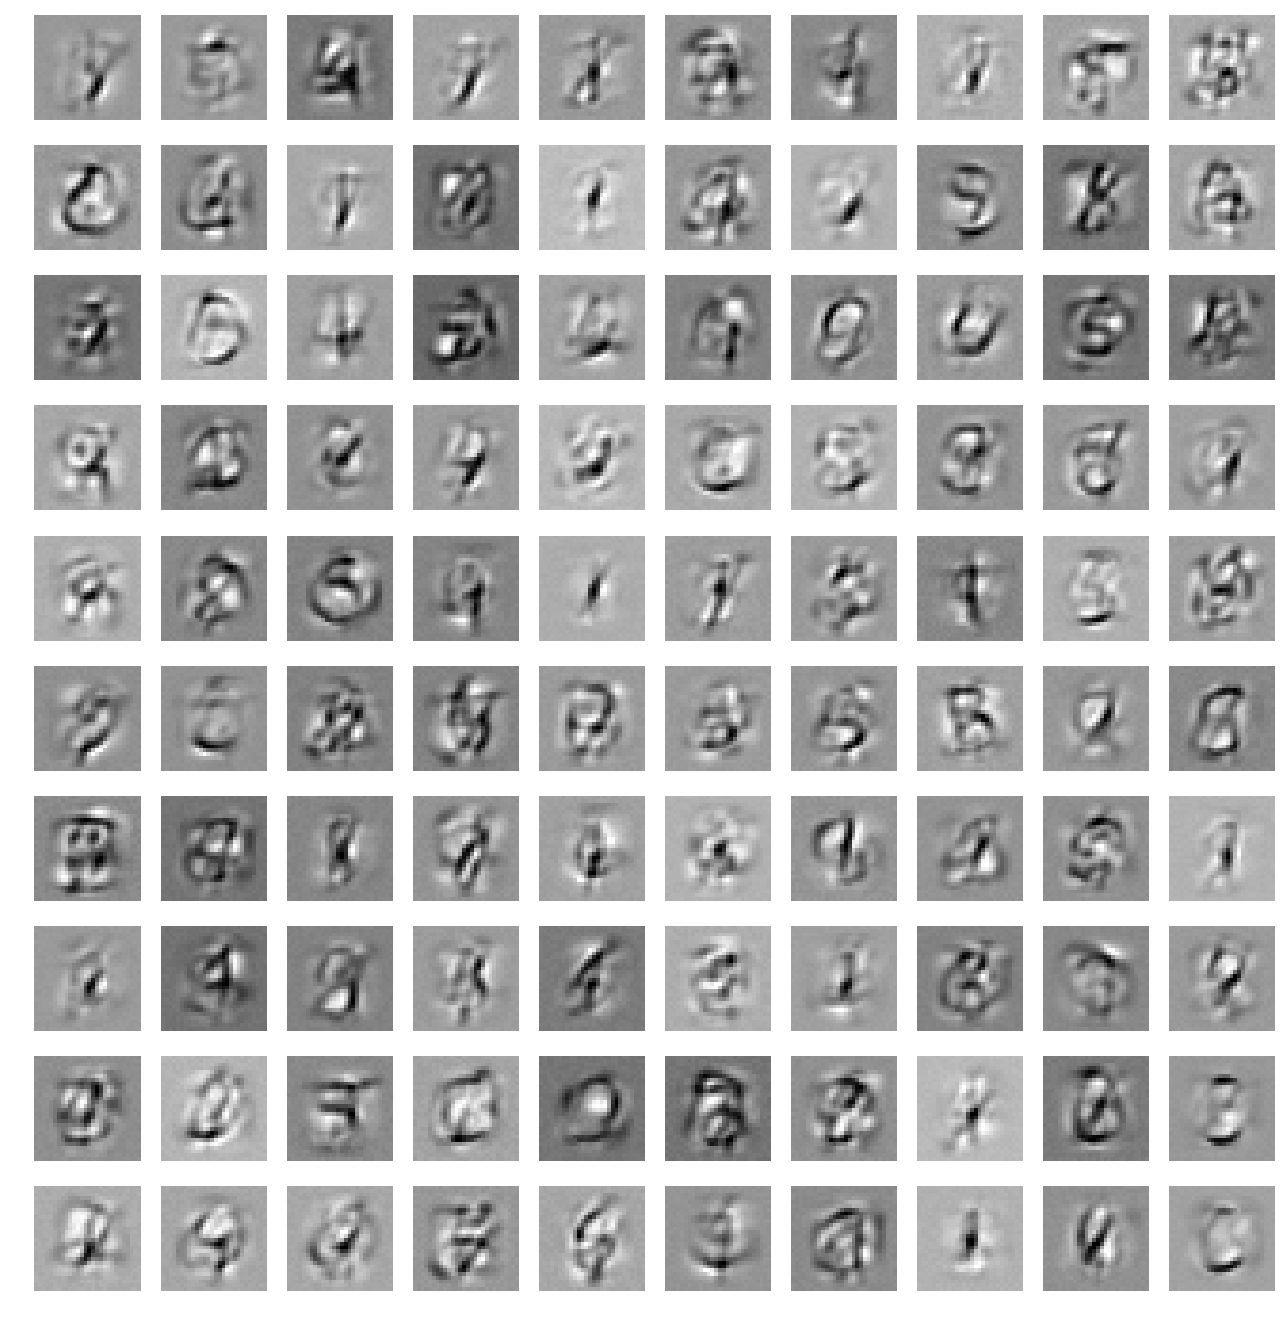
\includegraphics[width=0.8\linewidth]{experiment3_1.png}
	\caption{Visualization of the filters of the first 100 hidden nodes in an
	denoising autoencoder trained over all 60000 images.}
	\label{fig:experiment3_1}
\end{figure}

We first analyze how the number of threads affects the rate at which training
error decreases. We train a single autoencoder layer with 500 hidden nodes for
15 iterations over 5000 training images. An iteration involves going through
all training images and for each image, use SGD to update the weight matrix.
Fig.~\ref{fig:experiment1} shows the relationship between training error, total
time elapsed, and the number of threads used. Regardless of the number of
threads, the training error decreases sharply in the first few iterations
before flattening out to around the same value after 15 iterations. The rate at
which error decreases is significantly faster for four and eight threads when
compared to just using one. Nonetheless, the speedup is not linear and is due
to two reasons: 1) Possible cache conflicts as each thread read and writes to
different locations in the weight matrix. 2) All the steps for
backpropagation/SGD, described in Algorithm \ref{alg:backprop}, must be done
sequentially. Parallelization can only be done within each step and incurs an
overhead cost.

\begin{figure}[h]
\centering
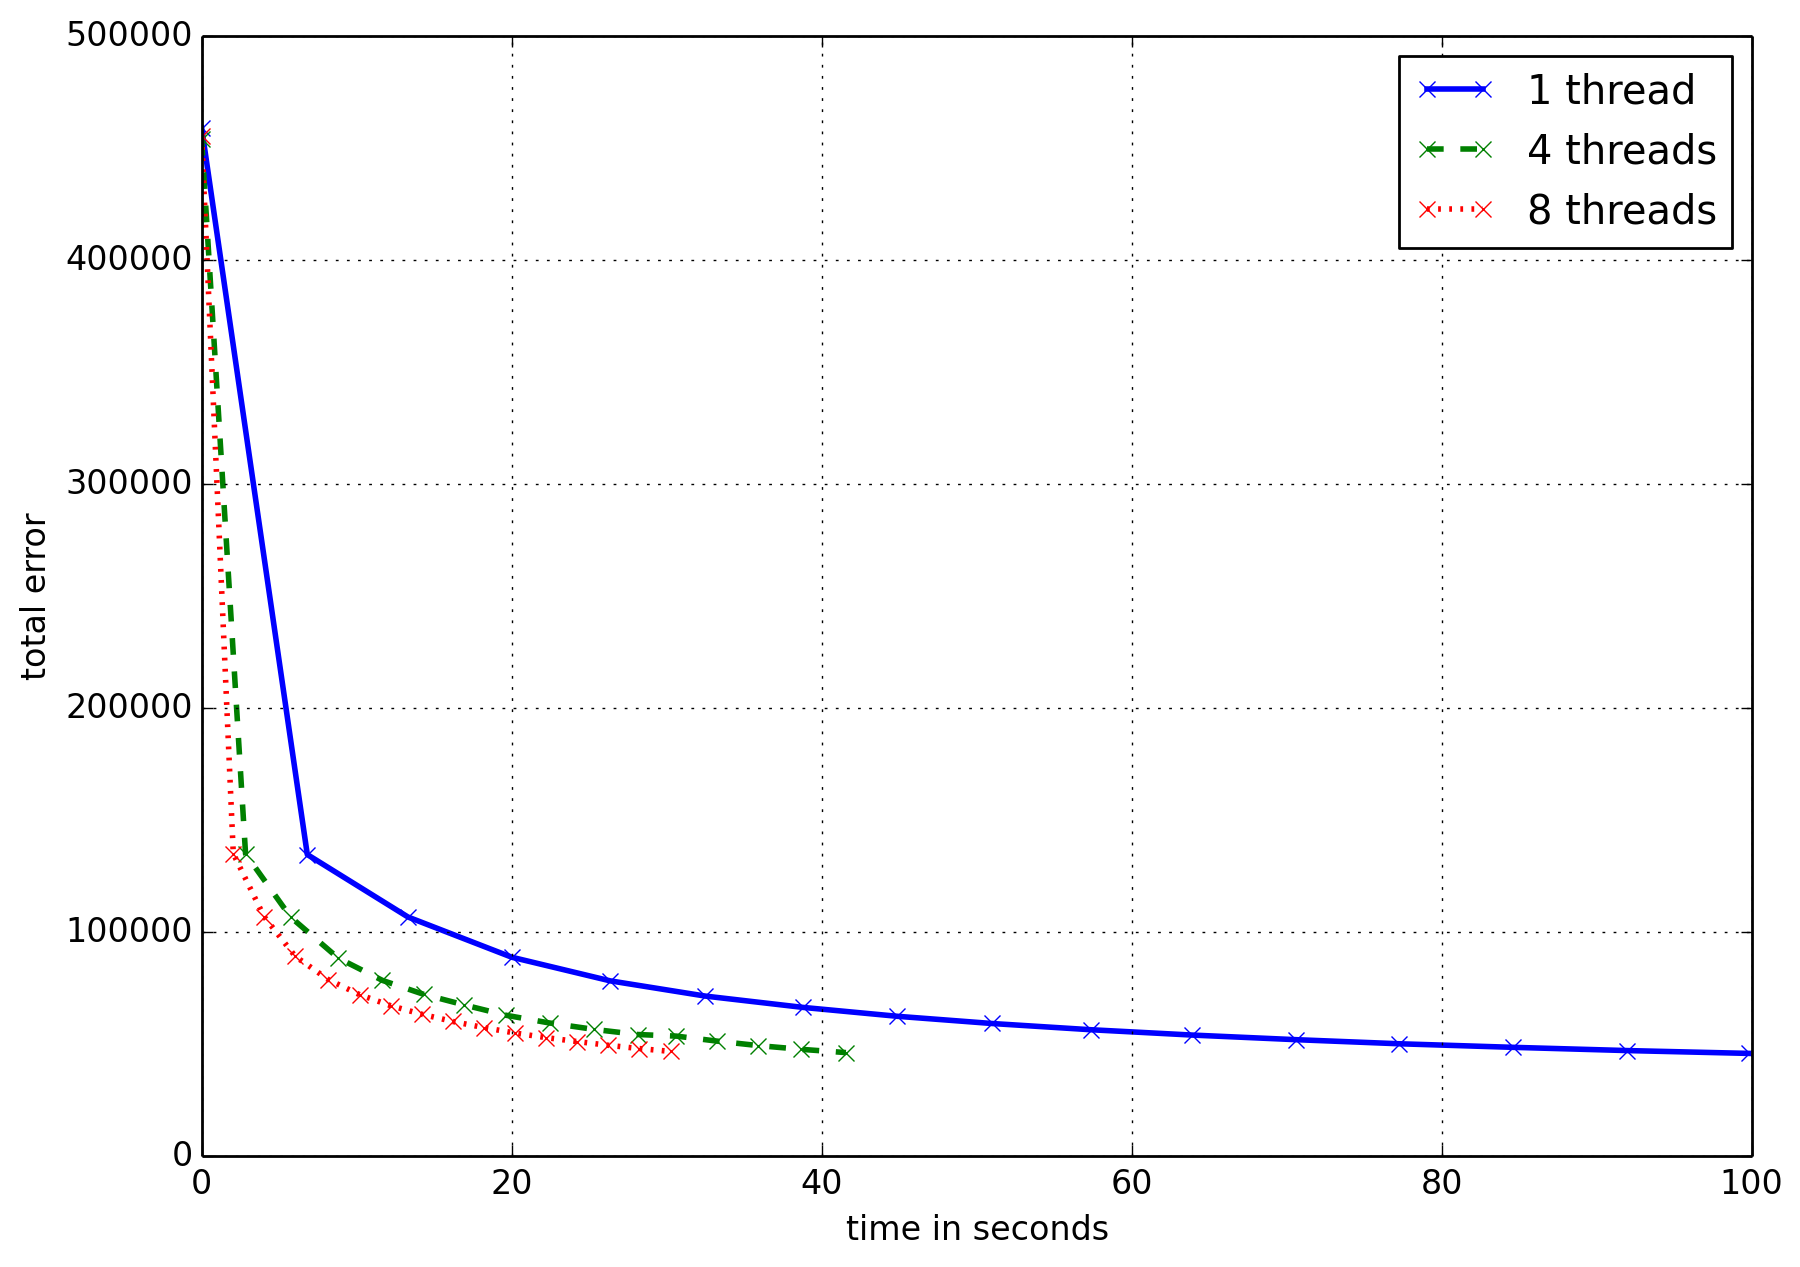
\includegraphics[width=0.8\linewidth]{experiment1.png}
\caption{Performance results on a single autoencoder layer with 500 hidden nodes and trained for 15 iterations. Plot shows time elapsed versus total training error over 5000 images for 1, 4, and 8 threads.}
\label{fig:experiment1}
\end{figure}


We note that the steps of backpropagation can only be done in sequence; thus we can only parallelize the operations done within each step. The three major operations which benefit from parallelization are computing the matrix-vector products $W^{H}x$ and $W^{O}y$, computing $\delta^O_j$ and $\delta^H_j$, and updating the entries of the weight matrices with the gradient. For performance reasons we dont store $W^O$ separately; instead we access $W^H$ with transposed indexes when decoding, calculating $\delta^O_j$, and applying the gradient update.

The most expensive parts of the backpropagation algorithm are computing the forward activations of the network and updating the weight matrices for the network. Computing the forward propagation requires performing a matrix-vector multiplication at each layer of the network. The size of that matrix depends on the input and output sizes of that layer. Thus if we have a network with $N$ layers and the sizes of each of those layers is $n_i$, then We have $N$ matrix-vector multiplications of size $n_{i-1} \times n_i$. Updating the weights also has complexity based on the size of the matrix since it requires updating all the entries of the matrix at each iteration.

To improve the performance of these two expensive steps, we parallelized them first using OpenMP and then later parallelized the matrix-vector products using OpenBLAS. Parallelization of these two steps is fairly straight forward and we give some results on scaling in Figs.~\ref{fig:performanceomp},~\ref{fig:performanceblas}, and \ref{fig:ompvsblas}.


\begin{figure}[h]
\centering
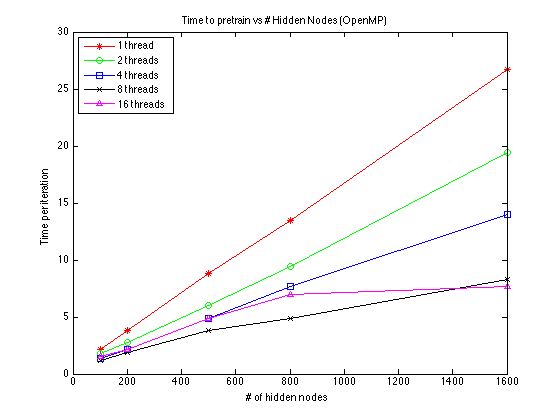
\includegraphics[width=0.8\linewidth]{performanceomp.png}
\caption{Time per iteration versus the number of threads and hidden nodes. We use our own parallel implementation using OpenMP and we use 5000 training images.}
\label{fig:performanceomp}
\end{figure}


\begin{figure}[h]
\centering
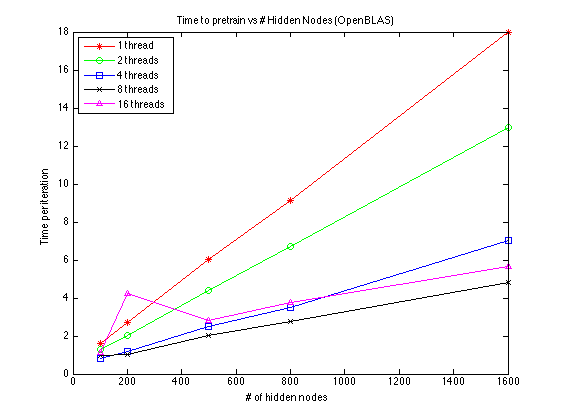
\includegraphics[width=0.8\linewidth]{performanceblas.png}
\caption{Time per iteration versus the number of threads and hidden nodes. We parallelize with OpenBLAS and we use 5000 training images.}
\label{fig:performanceblas}
\end{figure}

\begin{figure}[h]
\centering
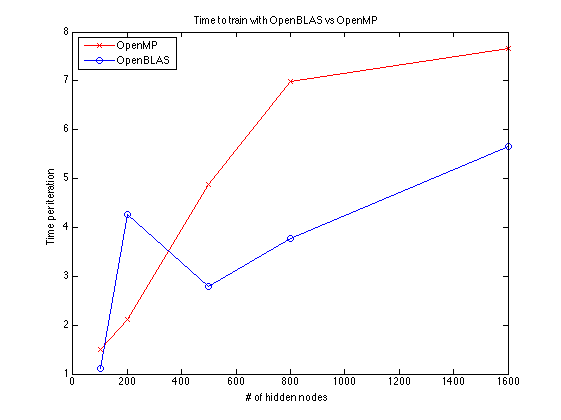
\includegraphics[width=0.8\linewidth]{ompvsblas.png}
\caption{Time per iteration versus parallelization technique and hidden nodes. We use 16 threads here.}
\label{fig:ompvsblas}
\end{figure}

In  Fig.~\ref{fig:performanceomp} we give the performance of training the autoencoder using SGD for different numbers of hidden nodes and different numbers of threads using our own parallel implementation.
In  Fig.~\ref{fig:performanceblas} we give the performance of training the autoencoder using SGD for different numbers of hidden nodes and different numbers of threads using OpenBLAS for parallelization of the matrix-vector multiplies and
matrix-transpose-vector multiplies. The weight updates are not able to be done in OpenBLAS, and so we continue to do that using OpenMP.
We consider the relative performance of these two methods in Fig.~\ref{fig:ompvsblas}.

We note that Figs.~\ref{fig:performanceomp} and~\ref{fig:performanceblas} show similar scaling, though in most cases the OpenBLAS version outperforms our own implementation. However, for small numbers of nodes, OpenBLAS does not perform well with many threads.

We generally get increasing amounts of speedup with increasing number of threads, but with a large number of threads we do not see improvement until the problem size increases and becomes large enough. We do not achieve linear scaling (i.e. twice as many threads does not result in the algorithm running twice as fast), since not all parts of the algorithm are parallelizable. That said, our algorithm does continue to get faster with increasing number of threads.





\subsection{Visualization of Autoencoder}

Next, in Fig.~\ref{fig:experiment3_1}, we visualize the filters that are
learned by training an autoencoder layer with 500 hidden nodes over all 60000
training images. The  filter for each hidden node is a row vector of the weight
matrix and indicates which aspects of the input the hidden unit is sensitive
to. Since each row in the weight matrix is the same dimensionality as the
input, we can visualize it as a 28 by 28 pixel image. The filters are not
identical to the input images, but do show some similarity to them. In
Fig.~\ref{fig:reconstruct}, we visualize the reconstructed digits when given
noisy test digits as input. The reconstructed outputs for most of the input
images are easily recognizable as digits, which indicates that the autoencoder
is indeed denoising and learning a good representation of the images.

To further demonstrate the reconstruction capabilities of the autoencoder, we
trained the autoencoder on corrupted or otherwise altered digits.  In
particular, we test the reconstruction on \textit{bg-rand}, which is generated
from the MNIST dataset, excpt that a random background is added. In
\textit{bg-img}, each image is given a background randomly selected from one of
twenty images downloaded form the internet. In \textit{rot}, the digits are
simply rotated by some random angle.  These alterations to the images make the
classification task more difficult. Indeed the digits are very difficult to
identify, but the autoencoder creates an easier to identify representation,
even to the human eye. We show also in Fig.~\ref{fig:reconstruct} the
reconstructed images form the \textit{bg-img} and \textit{rot} datasets. Note
that the images in the \textit{bg-rand} and \textit{bg-img} datasets are
rotated, but they are all rotated in the same way.



Finally we evaluate the classification accuracy of a deep neural network that
has multiple stacked denoising autoencoders. We train 3 stacked autoencoder
layers, each with 1000 hidden units, and using noise levels 0.1, 0.2, and 0.3
respectively. Each layer is trained for 15 iterations with a learning rate of
0.001. After the unsupervised pretraining, a conventional feedforward network
with 1000 input units, 500 hidden units and 10 outputs is connected to the
hidden units of the last autoencoder layer. This conventional network is then
trained for 30 iterations (learning rate 0.1) in a supervised manner, where the
target $t$ is the indicator vector representation of the training label. Our
final classification accuracy is 98.04\%. In comparison, the accuracy achieved
with a SVM with RBF kernel is 98.60\% \cite{vincent2010stacked}.

\subsection{Representation Learning for Supervised Classification}

Recall that one of the main reasons for using an autoencoder is to determine a
more useful representation of the data for other tasks, for example in a
classification task. To this end, we constructed and trained (15 iterations) an
autoencoder with just a single layer and 1000 hidden units and used it to
create a more useful representation of the digits in the MNIST dataset. After
this more useful representation is constructed, we can then use the output from
the autoencoder as input to another type of classification algorithm.  Since
the autoencoder produces a better representation of the data, we expect that
given the encoded data, the other classification algorithms should perform
better.  The results of these experiments is given in
Table.~\ref{tab:classvsenc}.

To test this,we used liblinear to attempt to train a model and then predict on
a test set for both the original and encoded datasets. With the original data
liblinear gives an accuracy of 91.68\% on the test set when using the default
parameters. However, when the encoded data from the trained autoencoder gives
an accuracy of 97.07\%. This is a nontrivial improvement in the classification
accuracy. Thus, the autoencoder has created a better representation of the data
which made it easier for liblinear to classify. This verifies that the
autoencoder is doing what it is expected to do.

Similarly, we performed the same experiment as above, except in this case we
used libsvm with an RBF kernel and all the default parameters.  Without
encoding the data first, we get an accuracy of 94.46\%, but using the encoded
data gives a prediction accuracy of 95.48\%. As above, the encoded data allows libsvm
better classify the data.

Using logistic regression to perform the classification, we experienced similar results.
Again we use liblinear with all default options except selecting logistic regression. Using the
original MNIST data, this algorithm achieved an accuracy of 91.82\% while with the encoded data
we achieved an accuracy of 96.86\%.

We performed the same experiments on the \textit{bg-rand}, \textit{bg-img} and 
\textit{rot} datasets as well. Across the board we see similar results. The encoding does not have much of
an effect on the ability of kernel SVM to classify the data, but for linear SVM and logistic regresssion, 
using the autoencoder always results in the classifier improving it's accuracy. 


\begin{table}[h]
	\centering
\begin{tabular}{ll|lll}
    Dataset                        & Data               & Linear SVM & Kernel SVM (RBF) & Logistic Regression \\ \hline
    \multirow{2}{*}{MNIST}         & Original           & 91.68\%    & 94.46\%          & 91.82\%             \\
                                   & Encoded            & 97.07\%    & 95.48\%          & 96.86\%             \\ \hline
    \multirow{2}{*}{mnist-bg-rand} & Original           & 58.975\%   & 83.875\%         & 65.5917\%           \\
                                   & Encoded            & 81.675\%   & 83.6583\%        & 83.825\%            \\ \hline
    \multirow{2}{*}{mnist-bg-img}  & Original           & 69.25\%    & 76.4667\%        & 71.6333\%           \\
                                   & Encoded            & 78.4333\%  & 72.8417\%        & 78.1333\%           \\ \hline
    \multirow{2}{*}{mnist-rot}     & Original           & 11.204\%   & 13.328\%         & 11.868\%           \\
                                   & Encoded            & 18.428\%   & 14.378\%         & 18.78\%
\end{tabular}
	\label{tab:classvsenc}
	\caption{Summary of the results of running different classification algorithms on the raw MNIST data and on the output from a trained autoencoder. We
	see in all cases that using the encoded data produces a better result.}
\end{table}





\begin{figure}[h] \centering
	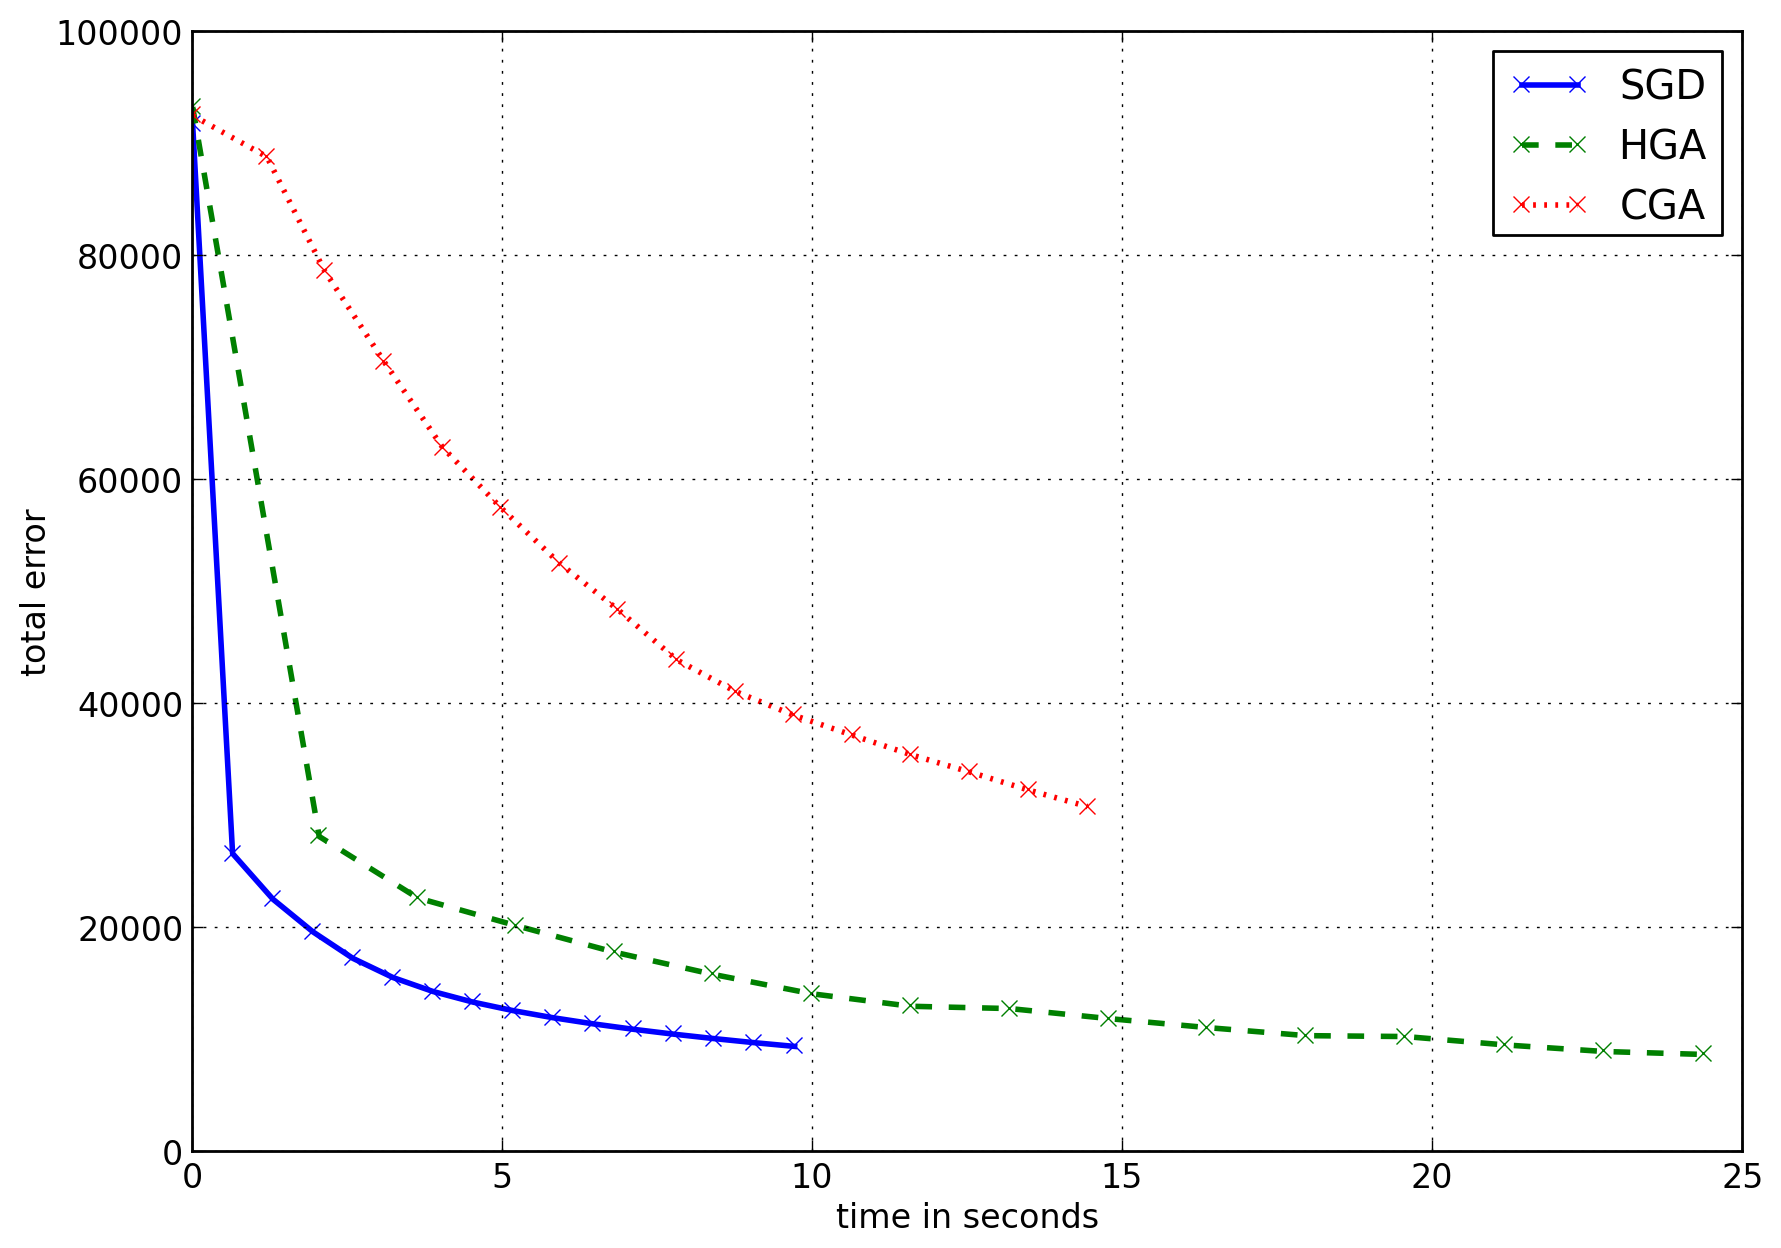
\includegraphics[width=0.8\linewidth]{ga_comparison.png}
	\caption{Comparison of the performance of SGD, HGA, and CGA. SGD is fastest, while HGA achieves the lowest reconstruction error.}
	\label{fig:ga_comparison}
\end{figure}

\begin{figure}[h] \centering
	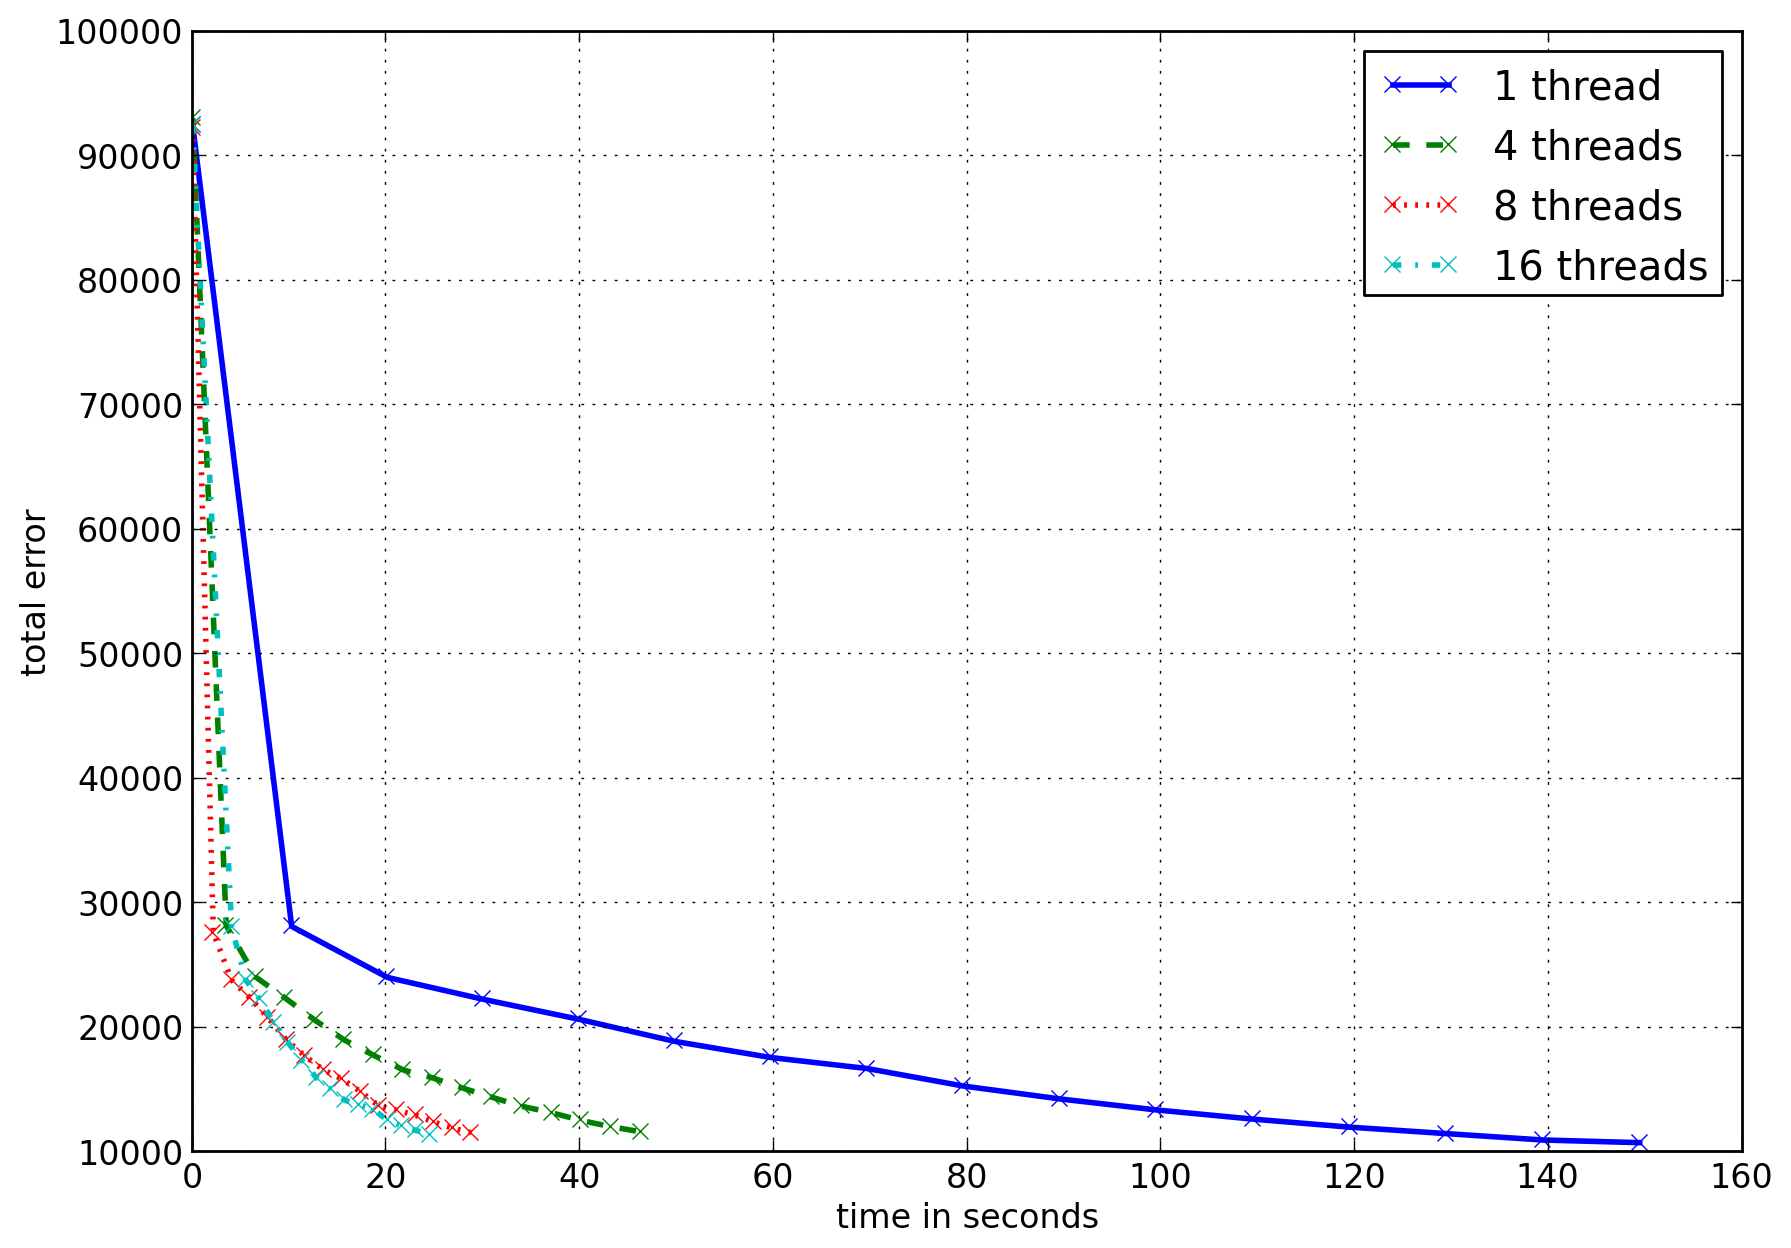
\includegraphics[width=1.0\linewidth]{ga_comparison2.png}
	\caption{Performance of HGA for 1, 4, 8, and 16 threads.}
	\label{fig:ga_comparison2}
\end{figure}

\begin{figure*}[h]
	\centering
	\subfloat[]{
		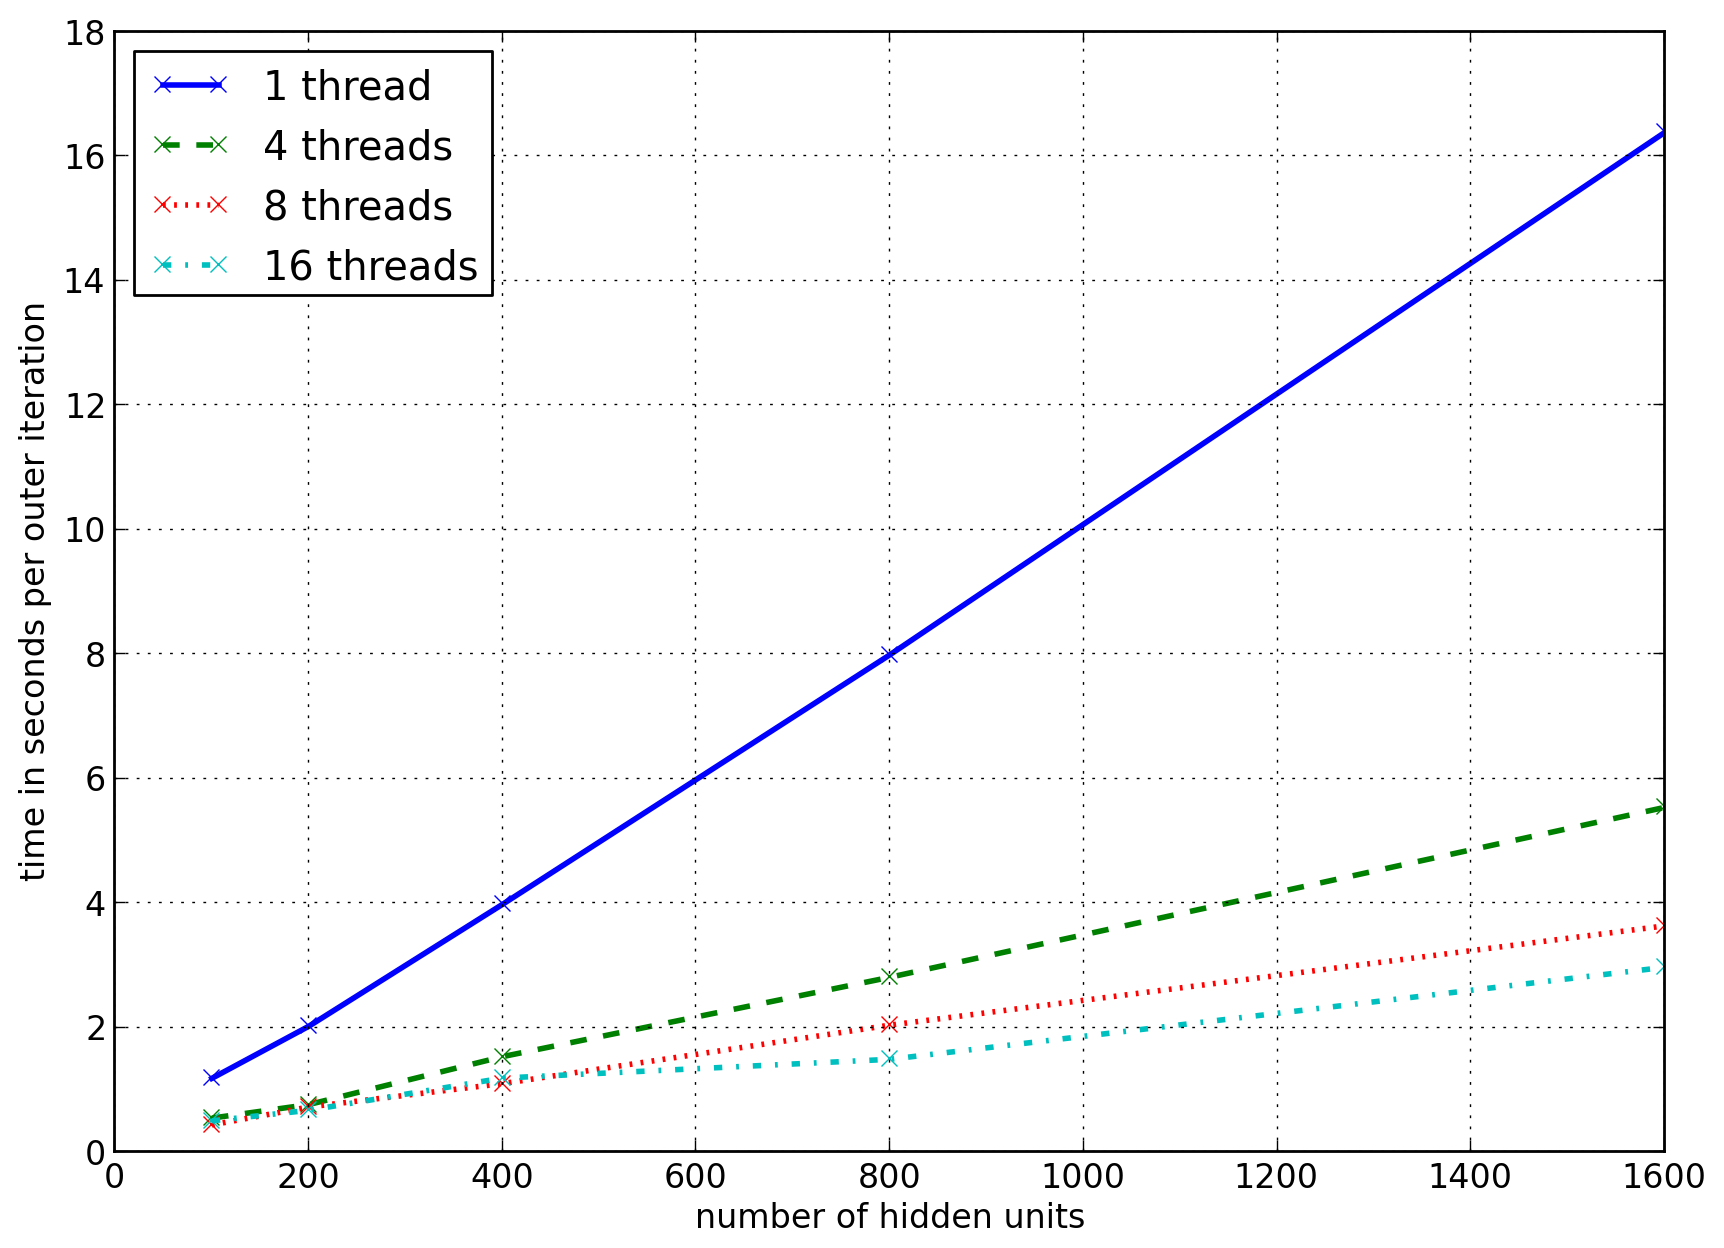
\includegraphics[width=0.4\textwidth]{ga_comparison3.png}
	}
	\subfloat[]{
		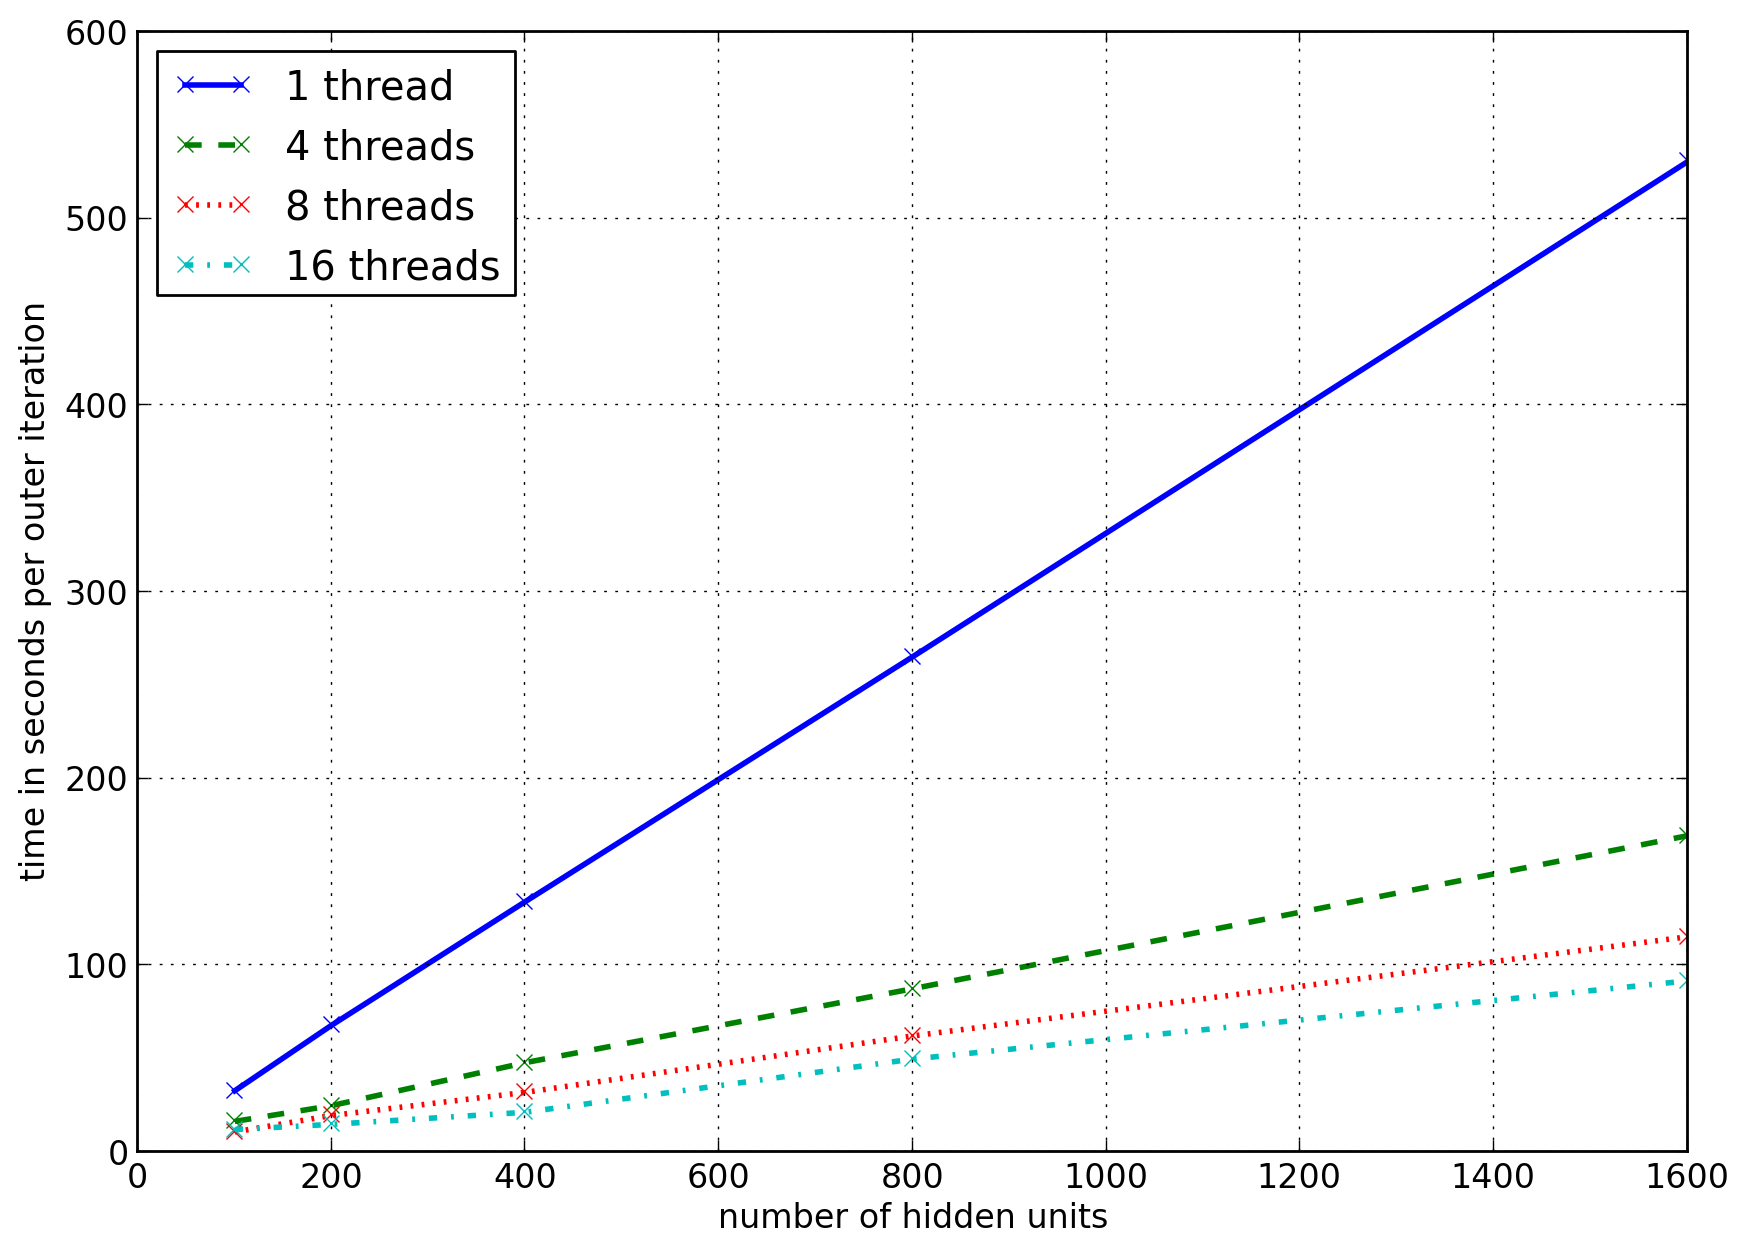
\includegraphics[width=0.4\textwidth]{ga_comparison3_big.png}
	}
	\caption{Comparison of performance versus number of threads and number of hidden units in autoencoder layer for HGA with population size (a) 2 and (b) 50.}
	\label{fig:ga_comparison3}
\end{figure*}

\subsection{Training the Autoencoder with a Genetic Algorithm}

In Fig.~\ref{fig:ga_comparison}, we compare the performance of stochastic gradient descent (SGD), our previously mentioned hybrid GA (HGA), which uses backpropagation to update the best individuals in the population, and a conventional GA (CGA), which does not use any gradient information. All three algorithms are used to train a single autoencoder layer with 1000 hidden units and cycle through 1000 training digits for 15 iterations. For SGD and HGA, we fix the learning rate to 0.0002. SGD is the fastest by roughly a factor of two when compared to HGA, while CGA is somewhere in between. However, HGA is able to achieve the lowest reconstruction error (8709 vs SGD's 9427). CGA performed the worst out of all 3 algorithms, having a reconstruction error that is three times larger than that of the other algorithms. The hyperparameters for HGA and CGA are hand tuned and not necessary optimal. However, we believe that will properly tuned hyperparameters, HGA might be competitive with SGD for both final reconstruction error and performance time. 

Next in Fig.~\ref{fig:ga_comparison2}, we examine the scalability of HGA. HGA shows roughly 3x speedup when using 4 threads, 5x speedup when using 8 threads, and 6x speedup when using 16 threads. The performance improvement versus the number of threads is sublinear and can be attributed to two main causes: 1) Cache conflicts when performing mutation and crossover due to multiple threads writing and reading different memory locations, 2) The sequential nature of backpropagation, which HGA utilizes to help optimize the weights. However, we do see that HGA does seem to moderately better scalability than our parallel implementation of SGD. This is attributable to the fact that the mutation and crossover operators are very straightforward to parallelize and scale in performance very well. 

In Fig.~\ref{fig:ga_comparison3}, the performance of HGA versus the number of threads and number of hidden units in autoencoder layers is visualized for both when HGA has a population size of 50 and its default population size of 2. As we can see, the HGA's performance scales linearly with the number of hidden units and that this relationship holds even when the population size is increased to 50. Interestingly, the performance when using 8 or 16 threads is not distinguishable for small numbers of hidden units. This is probably due to the overhead that result from creating additional threads.

Finally, in Fig.~\ref{fig:ga_comparison4}, we see how the performance of HGA and CGA scales versus the population size. All other hyperparameters remain the same for both HGA and CGA. As we can see, increasing the population does not lead to any noticeable improvement in reconstruction error per iteration. The default population size of 2 seems to be optimal. However, for CGA increasing the population does seem to lead a significant improvement in reconstruction error per iteration. Unfortunately, the overall running times when using increased population sizes are also larger. 


\FloatBarrier

% \FloatBarrier
\section{Discussion}
% \begin{figure*}
	\centering
	\subfloat[]{
		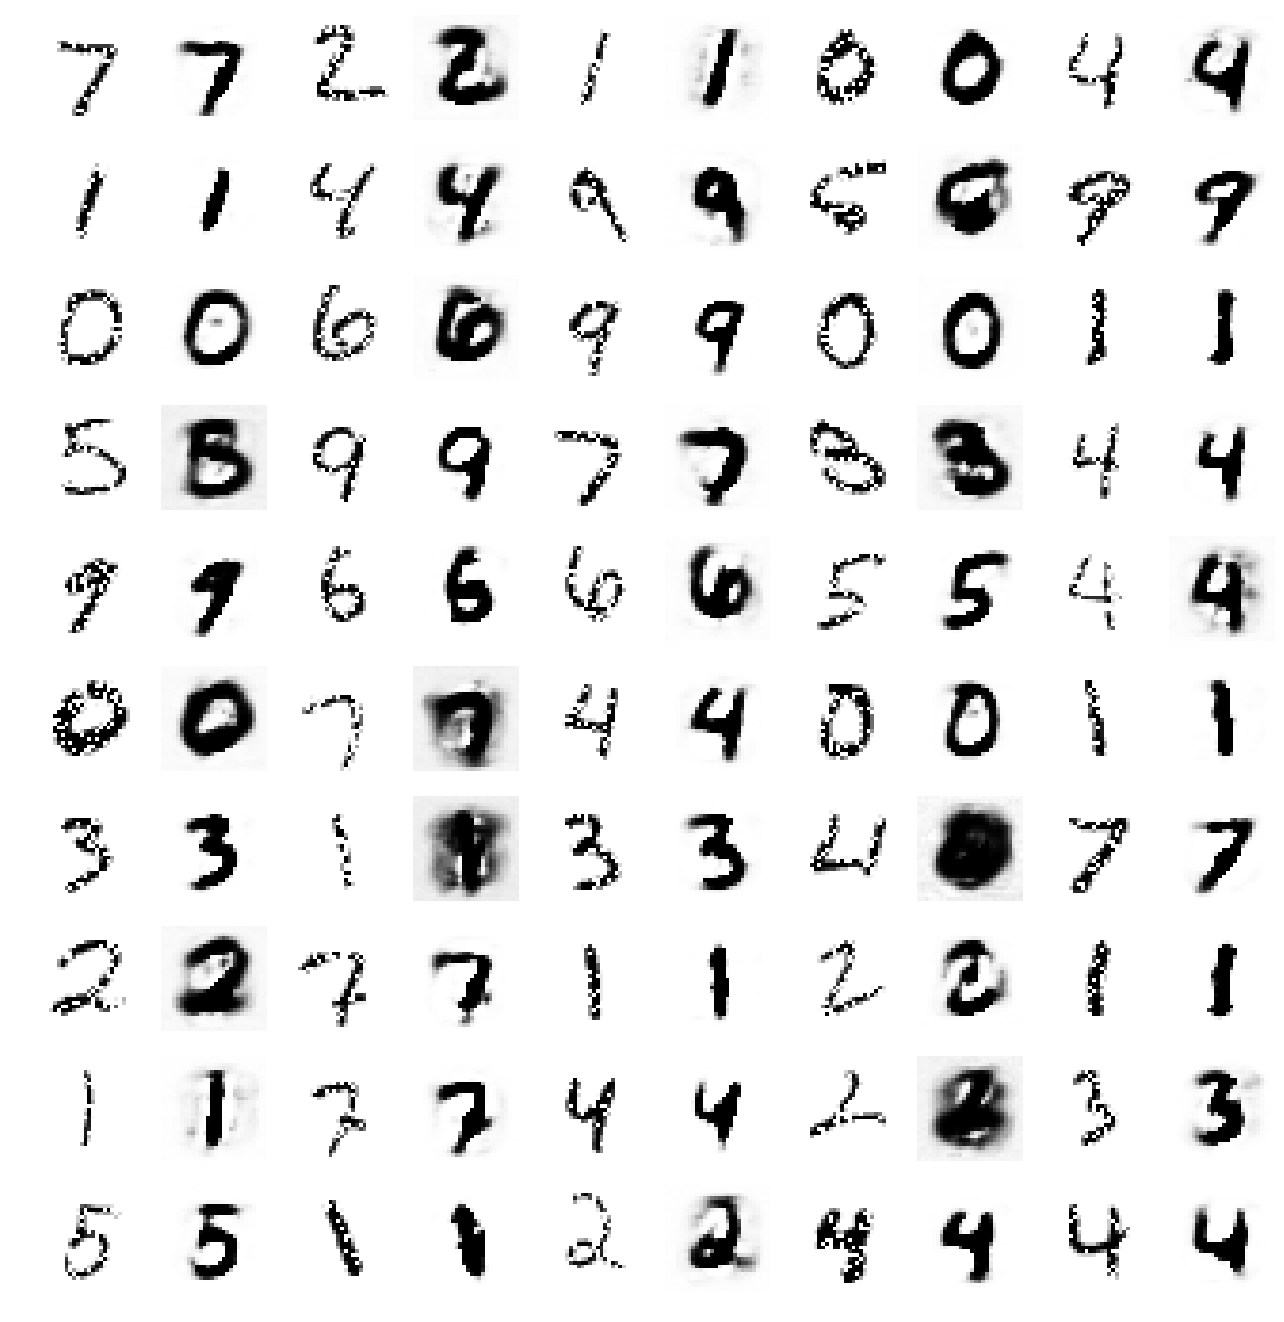
\includegraphics[width=65mm]{experiment3_2.png}
	}
	\subfloat[]{
		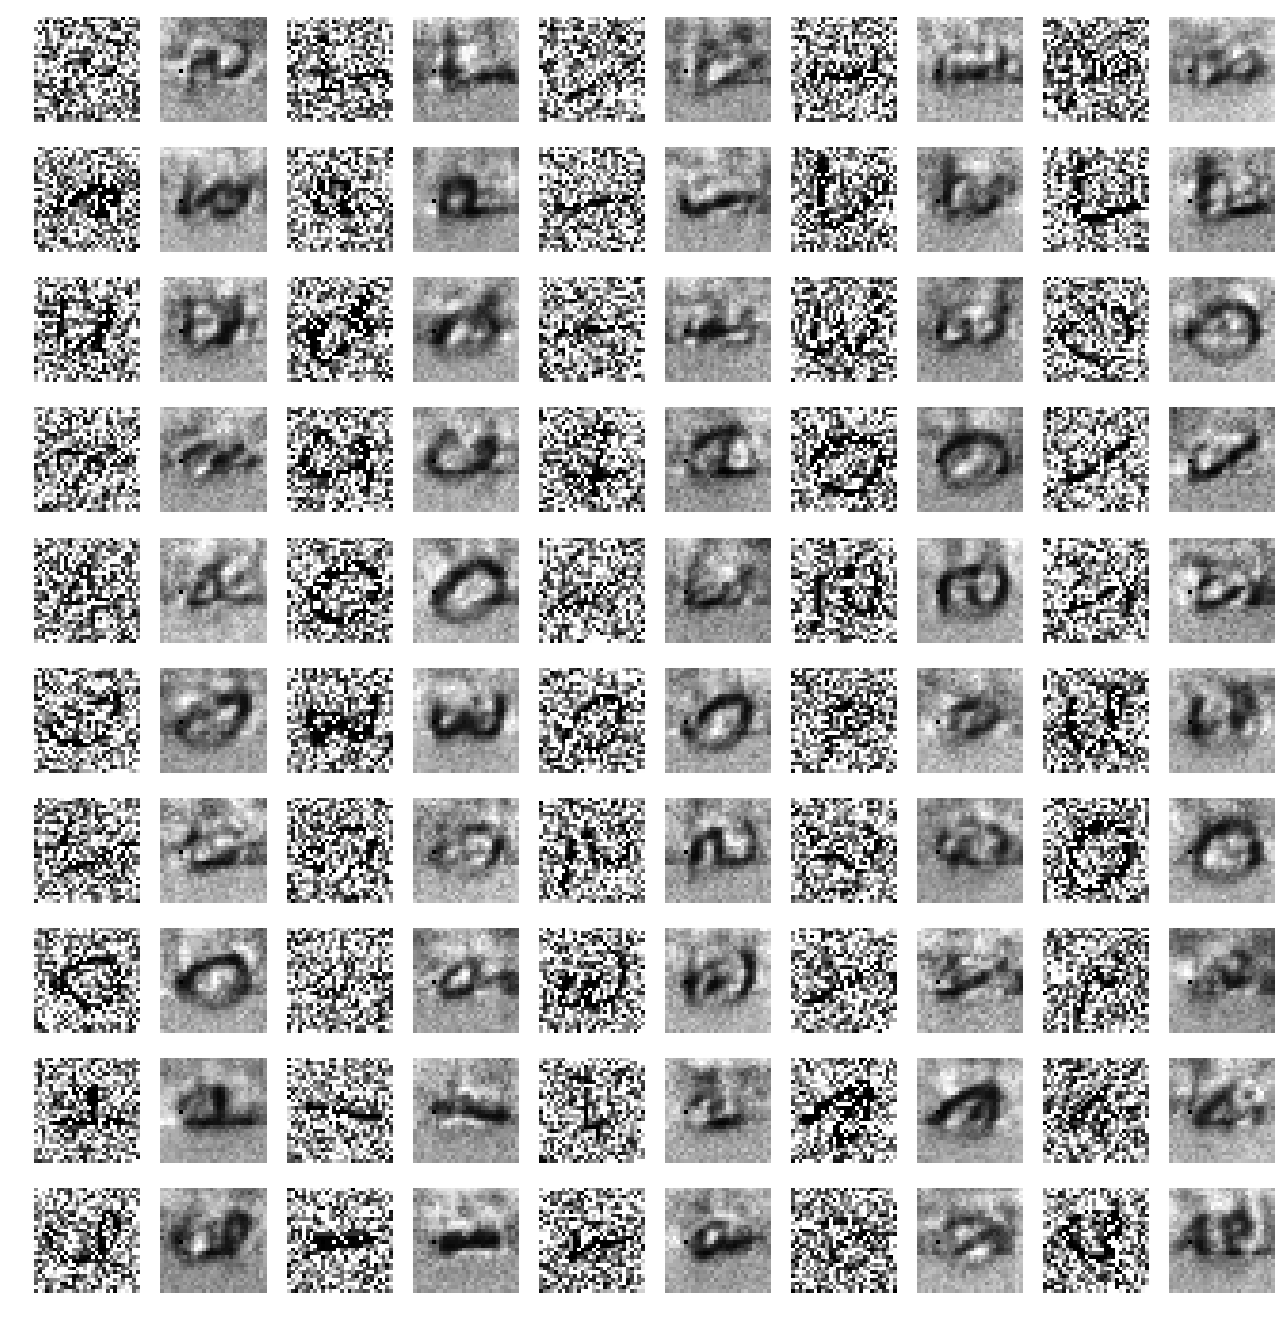
\includegraphics[width=65mm]{rand.png}
	}
	\hspace{5mm}
	\subfloat[]{
		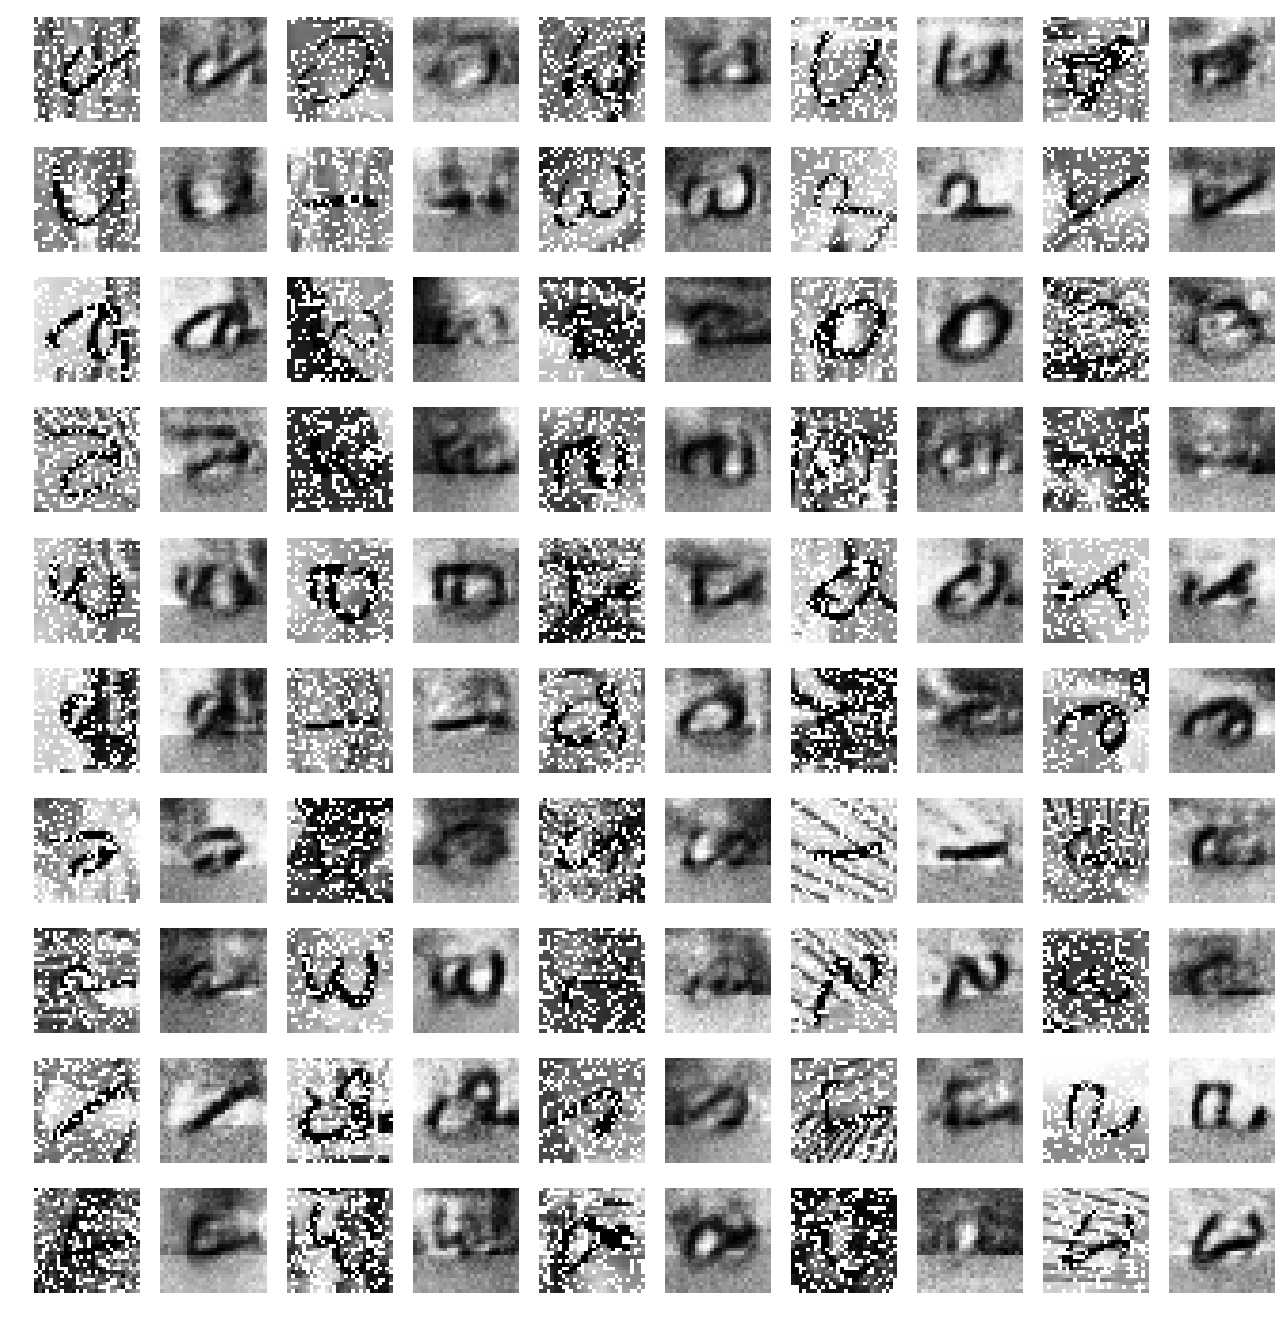
\includegraphics[width=65mm]{bg.png}
	}
	\subfloat[]{
		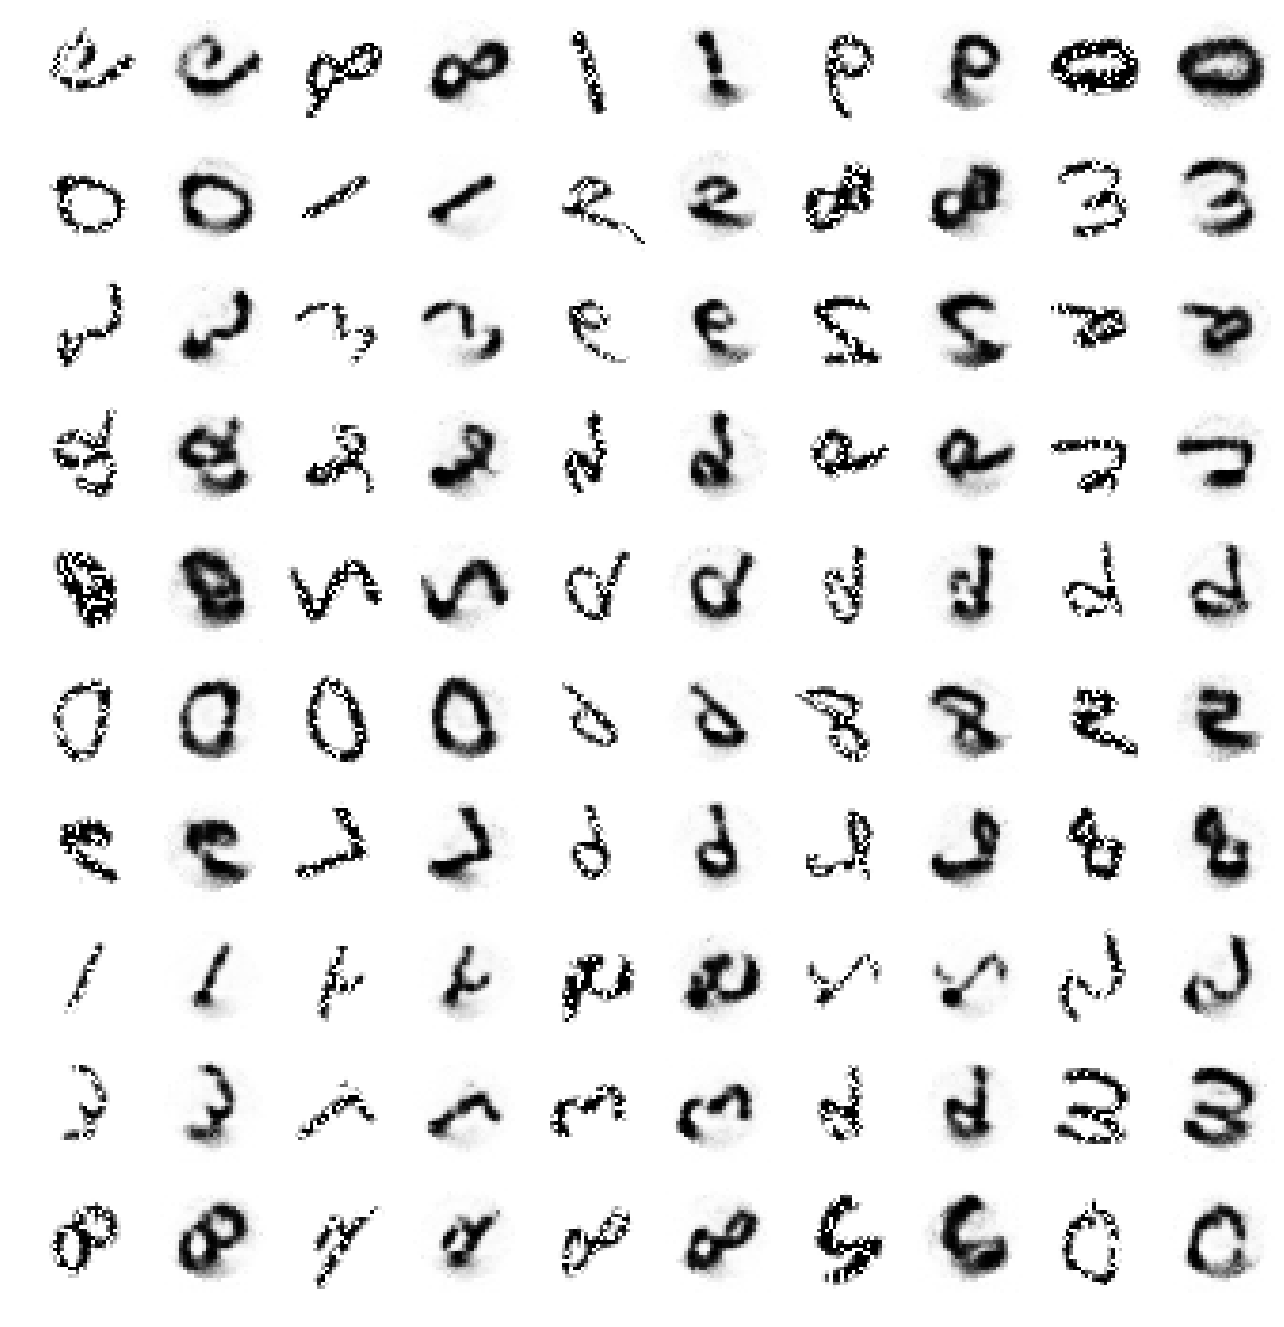
\includegraphics[width=65mm]{rot.png}
	}
	\caption{reconstructions of corrupted digits from the (a) MNIST dataset (b) bg-rand dataset, (c) bg-img dataset, and (d) rot dataset}
	\label{fig:reconstruct}
\end{figure*}

The experimental results demonstrate the importance of learning a better representation of the data for the classification algorithms given. While the kernel SVM performed comparably with and without the improved representation of the data, it is also much more expensive than the linear SVM or logistic regression methods. Thus the trade off becomes whether to use a more expensive classifier, or to learn a better representation and then use a cheaper classifier. It is also important to consider that the autoencoder combined with a simple classifier performed better than the kernel SVM in several cases.

As we saw in the results section, SGD is the fastest method for training the autoencoder, in terms of walltime. That is, to achieve a given error rate, using SGD will be faster than HGA or CGA in terms of time (as opposed to number of iterations). This might suggest that SGD is the preferred method for training an autoencoder, but it does not come without drawbacks. In terms of the number of iterations to achieve a given error rate, we saw that HGA performed the best, with SGD second and CGA last. This is important because of how the methods scale. SGD scales decently with respect to increasing number of threads, but the genetic algorithms demonstrate better scaling properties, being closer to linear in their scaling. 
Furthermore, HGA is able to achieve the lowest error rate of any of the methods considered. Reconstruction error is an indication of of how well the autoencoder encodes (and decodes) the input; by this metric HGA is a better optimization method than SGD.

However, genetic algorithms have many parameters that need to be tuned and are problem dependent. In contrast, SGD has only one: the learning rate. Consequently it can sometimes be difficult to get GAs to converge at all or at a reasonable rate without knowing the correct parameters. Thus it may be interesting to consider a metaoptimization of the parameters for a genetic algorithm, so that this tuning may be done automatically. 


% \FloatBarrier
\section{Future Work}
%%%%%%%%%%%%%%%%%%%%%%%%%%%%%%%%%%%%%%
%% Frame
%%%%%%%%%%%%%%%%%%%%%%%%%%%%%%%%%%%%%%

\begin{frame}[t]
	\frametitle{Future Work}
	\framesubtitle{~~}  %% needed for proper positioning of the logo ...
	\begin{itemize}
		\item Metaoptimization of the parameters for genetic algorithms
		\item Adaptive genetic algorithm for optimization
		\item Distributed parallelization of SGD or GAs for autoencoders
	\end{itemize}

\end{frame}



% \FloatBarrier
\section{Conclusion}
We have implemented stacked denoising autoencoders and shown that it achieves accuracy comparable to state of the art classifiers like a SVM with RBF kernel. We also have shown that our autoencoder layers are learning good representations and are capable of denoising and reconstructing the input with little error. These learned representations improve the ability of other classification algorithms to correctly classify the data. We find that SGD scales well with increasing number of hidden units and with increasing number of threads. Lastly, we discovered that HGA, a genetic algorithm that makes use of gradient information, is competitive with SGD, and scales just as well if not better with the size of the autoencoder and number of threads. 

\FloatBarrier

\bibliographystyle{unsrt}
\bibliography{autoencoder}

\end{document}


